\documentclass[12pt, titlepage]{report}
\usepackage{consumer_resource_final}
\graphicspath{{./figures/Results/feasibility}}

\begin{document}
As explained in Methods \ref{sec : methods feasibility}, before addressing the question of the stability of a system, be it dynamical or structural, it is important to study whether that system is \important{feasible}. In short we must answer the question: ``does it make sense to talk about this system? What are the restrictions on the parameters of a microbial community in order for it to exist?''.
 Methods \ref{sec : methods feasibility basic concepts} provides a mathematical definition of \important{feasibility}. Intuitively, we say that in order to be feasible, a microbial community should respect two conditions: biomass must be conserved and its parameters must have a direct biological interpretation. Methods \ref{sec : methods feasibility volume} defines $\forall x \in [0,1]$ the $x$-feasibility region $\mathcal{F}^{G,A}_x \subset \mathcal{M}$ of the consumption-syntrophy network $(G, A) \in \mathcal{B}_{N_S \times N_R} \times  \mathcal{B}_{N_R \times N_S}$. The idea behind that concept is that every metaparameter set $m \in \mathcal{M}$ contained in the $x$-feasibility region $\mathcal{F}^{G,A}_x$ gives rise to a percentage $x$ of feasible systems. Knowing where the different $x-$feasibility regions are located allows us to predict relationships between the different parameters of microbial communities. In particular, we would like to know which metaparameters $(\gamma_0, S_0, \alpha_0)$ yield through the algorithmic procedure $\mathcal{A}$ a hundred percent of the time a feasible parameters set. In short, we are interested in $\mathcal{F}^{G,A}_1$. A direct study of every triplet $(\gamma_0, S_0, \alpha_0)$ is difficult so we take a more ``implicit'' path in which we  determine, as a function of $\alpha_0$, what values $(\gamma_0, S_0)$ can take such that $m=(\gamma_0, S_0, \alpha_0)$ is in $\mathcal{F}^{G,A}_1$.


\subsection{The feasibility region in the absence of syntrophy}\label{sec : feasibility without syntrophy}

We start with the ``null'' case and study feasibility in the absence of syntrophy. A first order approximation of the fully feasible volume $\mathcal{F}^{G,A}_1$ is given by Eq.\eqref{eq : fully feasible volume}.
% , which we recall here:
% \begin{equation}
% \max_i\left\{\frac{\deg(A,i)}{\deg(G,i)}\right\} \alpha_0
% \lessapprox \min(1-\sigma_0, \sigma_0) \gamma_0 R_0
% \lessapprox
% \min \left(1-\sigma_0, \sigma_0 \right) \min_\nu \left\{ \frac{l_0}{\deg(G,\nu) S_0} + \frac{\deg(A,\nu)}{\deg(G,\nu)}\alpha_0\right\}.
% \end{equation}
In the absence of syntrophy $\alpha_0=0$, it becomes:
\begin{equation}
\gamma_0 R_0 \lessapprox \frac{l_0}{\max_\nu\{\deg(G,\nu)\}S_0}. \label{eq: fully feasible volume no syntrophy}
\end{equation}
That relation provides a lot of biological insight about how the different metaparameters of actual microbial communities should be linked together:
\begin{itemize}
\item For a fixed consumption interaction (\ie constant $\gamma_0$ and $G$) and average consumers abundance $S_0$, increasing the average resource equilibrium abundance $R_0$ implies increasing the external resource input rate. This is completely expected: since the microbes consume some part of the resources, more available resources can only come from outside in the absence of syntrophy.
\item For a fixed consumption network $G$, resources abundance $R_0$ and resource input rate $l_0$, a larger range of possible consumption rate $\gamma_0$ is possible if the consumers abundance is decreased. Since there are fewer the consumers, they can individually eat more from the available resources.
%\item the consumer equilibrium abundance $S_0$ increases. What this means is that if you want to maintain the same consumption interaction but get a higher abundance of resources at equilibrium, you must at the same time decrease the consumers equilibrium abundance.
\item For every metaparameter except $\gamma_0$ fixed, arranging the shape of $G$ such that few consumers eat from the same resources\footnote{Indeed, $\deg(G,\nu)$ is the number of species that consume resource $\nu$. Reducing the number of consumers that eat from the same species reduces $\max{\deg(G,\nu)}$ in Equation \eqref{eq: fully feasible volume no syntrophy}.} increases the range of possible consumption rates. If the total amount of resources is fixed, consumers can individually eat more of it if they do not have to share it!
%\item the largest column-degree of the consumption matrix decreases. The degree of a given column $\nu$ of the consumption matrix tells you how many species eat from resource $\nu$. This encourages communities of specialists, where each consumer eats from its own and no other resource.
\end{itemize}
%Overall we see that feasibility increases when the \important{consumption flow} $\simeq \gamma_0 S_0 \deg(G,\nu) $ is low $\forall \nu$.
Equation \eqref{eq: fully feasible volume no syntrophy} can be confronted to simulations.
The first step is to note that for all the matrices in the set we chose \textbf{TO DO: give a name to the matrix set}, there exists a fully feasible zone, \ie $\mathcal{F}^{G, 0}_1(\alpha_0=0) \neq \{\}$ $ \forall G$. There exists an overlap between all these regions $\mathcal{F}_1^{S_{25}}(0) \defined \intersection{G \in G_{25}} \mathcal{F}^{G,0}_1 \neq \{\}$, such that the critical feasibility $f^*(S)=1$ and the critical feasibility region at no syntrophy is the common fully feasible volume $\mathcal{F}_1^{G_{25}}$ (see Eqs.\eqref{eq : feasibility methods critical common feasibility} and \eqref{eq : feasibility methods critical common feasibility region}) \textbf{TO DO: add figure of this?}.

Figure \ref{fig: typical feasibility region} shows the typical proportion of feasible systems without syntrophy %$\mathcal{F}\left((\gamma_0, S_0, 0), G, 0\right)$ and $R_0=l_0=1$, $\sigma_0=0.25$ (see Methods \ref{sec : methods feasibility volume}),
for two consumption matrices $G_1$ and $G_2$ in the set $G_{25}$.
%of our set. $G_1$ has connectance $\kappa_1=0.17$ and nestedness $\eta_1=0.2$, $G_2$ is more connected and more nested: $\kappa_2=0.37$ and $\eta_2=0.4$.
We generally observe two distinct zones in the $(\gamma_0, S_0)$ space: full feasibility ($\mathcal{F}\left((\gamma_0, S_0, 0), G, 0\right)$ as defined in Eq.\eqref{eq : feasibility methods feasibility metaparameters function} is equal to $1$) and full infeasibility ($\mathcal{F}\left((\gamma_0, S_0, 0), G, 0\right)=0$). These two zones are separated by a narrow region of partial feasibility $0 <\mathcal{F}\left((\gamma_0, S_0, 0), G, 0\right)<1$. Since that region is very thin, we can define  the ``boundary'' line between feasibility and infeasibility as the level\footnote{Numerically because of the possible noise, we take as part of the boundary every $(\gamma_0, S_0)$ such that $0.4 < \mathcal{F}\left((\gamma_0, S_0, 0), G, 0\right)<0.6$.} $\mathcal{F}\left((\gamma_0, S_0, 0), G, 0\right)=0.5$. Theoretically, that sharp transition between feasibility and infeasibility happens when both sides of the inequality \eqref{eq: fully feasible volume no syntrophy} are equal, \ie at $\gamma_0 R_0 = l_0/\max_\nu\{\deg(G,\nu)\}S_0$. Hence we expect the boundary measured above to be well characterized by the curve $S_0 = K \gamma_0^{-1}$ with $K=l_0/(R_0 \max_\nu\left\{\deg(G,\nu)\right\})$.

 For $G_1$, the theoretical expectation is $S_0 = 0.125 \gamma_0^{-1}$ and a fit on the numerical results gives $S_0=(\num[scientific-notation=false]{0.124}\pm\num{3e-8}) \gamma_0^{-1}$ so the theoretical estimate is very accurate.
For $G_2$, we expect $S_0 = 0.077 \gamma_0^{-1}$. A fit gives $S_0=(\num[scientific-notation=false]{0.076}\pm\num{7e-9})\gamma_0^{-1}$. Again, the theoretical value is very close to the numerical measurement.
However, the numerical estimate does not always match the theoretical value that well. Figure \ref{fig: deviation away from theory feasibility} shows the relative error $\Delta_K \defined 1 - K_\text{theorical}/K_\text{fit}$. We see that in general $\Delta_K < 0$, \ie the theoretical expectation tends to overestimate the fully feasible region. This is probably due to noise (\ie coming from the difference between the metaparameters and the parameters) in the actual systems and the topology of the consumption matrix $G$. Figure \ref{fig: deviation away from theory feasibility} shows that the lower the ecological overlap or connectance of $G$, the worse the theoretical estimate. Finding a more accurate approximation which takes into account the deviations away from the metaparameters and the topology of $G$ remains a challenge for future studies.


We can similarly measure the common fully feasible volume in the absence of syntrophy $\mathcal{F}_1^{G_{25}}(0)$ (depicted in Fig.\ref{fig: common feasible volume no syntrophy}), which according to Eq.\eqref{eq: fully feasible volume no syntrophy} is inversely proportional to the largest maximal row degree of the matrix set. For the set $S_{25}$, this yields in theory: $S_0 = 0.053 \gamma_0^{-1}$. A fit on the points at the edge yields the critical boundary $S_0 = (0.042 \pm 10^{-8})\gamma_0^{-1}$, which is $\sim 21 \%$ away from the theoretical prediction. The discrepancy is probably due to the difference between the way we estimate the boundary numerically
and analytically.

\subsection{Impact of syntrophy on the feasible region}

Above we computed feasible volumes when there is no syntrophy \ie $\mathcal{F}^{G,0}_1$. Because there was no syntrophy, we did not need to specify what the structure of $A$ was. The next naturally arising question is then: what happens to the feasible region of a community with a given consumption matrix $G$ when we add a syntrophic interaction, \ie a syntrophic network $A$ of average interaction strength $\alpha_0$? More precisely, how does the shape of $\mathcal{F}^{G,A}_1$ change as a function of $A$ and $\alpha_0$?

A layer of complexity arises on top of the problem discussed above%. When we computed $\mathcal{V}^G_1(\alpha_0=0)$, we only had to take into account the structure of $G$, since there was no syntrophy. Now, we have an additional complexity because
: apart from the structure of the consumption matrix $G$, we now have to think about both the topology of $A$ and also $\alpha_0$ as well. As explained at the beginning of this section, studying in detail the topology of $A$ is too large of a scope for this study, so we focus on the four $A$ cases enunciated above (FC, NIS\textsubscript{1}, LRI\textsubscript{1}, RS\textsubscript{1}). Concerning the question of $\alpha_0$, we would like to be ``fair'' and study syntrophy strengths that are feasible for all the consumption-syntrophy networks considered $(G,A) \in S_{25}$.
  The largest common fully feasible syntrophy $\alpha_C^F(S_{25})$, which is the value of $\alpha_0$ such that $\mathcal{F}^{G,A}_1 \neq \{\}$ $\forall (G,A) \in S_{25}$, can be estimated with the help of Eq.\eqref{eq : fully feasible volume}:
  \begin{equation}
  \alpha_0 \lessapprox \frac{\min(1-\sigma_0, \sigma_0)\gamma_0 R_0}{\max_{(G,A)\in S}\left\{\max_i\left\{\frac{\deg(A,i)}{\deg(G,i)}\right\}\right\}} \approx 0.01 \gamma_0 \leq 0.01. \label{eq : results feasibility largest alpha0}
  \end{equation}
  We will hence investigate the impact of $\alpha_0$ evaluated at ten different values from $0$ to $0.015$. %We first consider the effect of syntrophic interaction on each consumption network $G$ then on the common fully feasible volume.
  Since we do not change $\alpha_0$ in a continuous way but instead focus on different ``$\alpha_0$-slices'' of $\mathcal{F}^{G,A}_1$, the object of our attention is the set of $(\gamma_0, S_0)$ such that $(\gamma_0, S_0, \alpha_0) \in \mathcal{F}^{G,A}_1$. In a rather unfortunate notation, we will refer to it as $\mathcal{F}^{G,A}_1(\alpha_0)$:
  \begin{equation}
  \mathcal{F}^{G,A}_1(\alpha_0) \defined \left\{(\gamma_0, S_0) : (\gamma_0, S_0, \alpha_0) \in \mathcal{F}^{G,A}_1 \right\}.
  \end{equation}
  Because Equation \eqref{eq : fully feasible volume} depends on the structure of $G$ and of $A$, we expect $\mathcal{F}^{G,A}_1(\alpha_0)$ to depend heavily on the topology of both the consumption and syntrophy matrices.

  \subsubsection{The influence of matrix topology}\label{sec : feasibility results influence of matrix topology}
  Figure \ref{fig: feasibility results fully feasible volume different consumption matrices} shows that indeed $\mathcal{F}^{G,A}_1(\alpha_0)$ changes significantly not only with syntrophy $\alpha_0$ but also with the network structure of the consumption matrix $G$. How $\mathcal{F}^{G,A}_1(\alpha_0)$ changes as a function of $A$ is a more difficult question. \textbf{TO DO: explain that this will be studied later : put reference to new figure (how do df and alpha0 change from the null case)?}

  We observe a general trend among all matrices: as syntrophy increases, the fully feasible region moves horizontally to the right towards a higher $\gamma_0$. This can be explained with Eq.\eqref{eq : fully feasible volume} which provides a lower bound to $\gamma_0$ when $\alpha_0 > 0$. Note that taking into account $\alpha_0 >0$ does not bound $S_0$, such that at a fixed $\gamma_0$, every $S_0$ from $0$ to the upper boundary critical curve $\sim \gamma_0^{-1}$ discussed before remains a fully feasible point. So in general, as syntrophy increases, systems with a high consumption rate and a low consumers abundance at equilibrium will remain feasible, while other simply will not exist. This makes sense intuitively:\textbf{TO DO: put explanation here}

  Because of that shift to the right,  $\mathcal{F}^{G,A}_1(\alpha_0)$ shrinks in size\footnote{Note that when we talk about the size of $\mathcal{F}^{G,A}_1(\alpha_0)$, it is understood relatively to the $(\gamma_0, S_0)\in [0,1]^2$ unit square.}: as syntrophy is increased, the set of possible consumption rate and average consumers abundance is more restricted.
  Figure \ref{fig: feasibility results typical shrinkage of feasible volume} shows that typically the feasibility volume $\text{Vol}\left(\mathcal{F}_1^{G,A}(\alpha_0)\right)$, formally defined in Appendix \ref{app: how to measure volume}, decays in an exponential-like fashion as $\alpha_0$ increases. This is a simple translation of the biological hindsight that, because of the physical considerations discussed above, the number of systems that can sustain a given syntrophic interaction strength decreases with that interaction strength, \ie no system can support an arbitrarily large syntrophy.
  The shrinkage of the feasibility volume can be quantified by defining the \define{feasibility decay rate} $d_F$, which is obtained by performing a non-linear regression to find the coefficients $c_1,c_2, d_F \in \mathbb{R}^+$ that satisfy best\footnote{In practice, standard functions of the \code{numpy} and \code{scipy} Python libraries are used to perform that fitting procedure.}:
  \begin{equation}
\text{Vol}\left(\mathcal{F}_1^{G,A}(\alpha_0)\right) \approx c_1 \exp{\left(-d_F \alpha_0\right)} - c_2. \label{eq: feasibility results fit feasible volume}
  \end{equation}
  The value of $d_F(G,A)$ tells us how fast the feasible volume shrinks for a given consumption-syntrophy couple $(G,A)$. In that sense $d_F(G,A)$ provides a measure of how good $(G,A)$ can sustain an increase in syntrophy\footnote{One could also desire to define a \define{critical feasible syntrophy} as the smallest syntrophy that gives a zero fully feasible volume. This would be a very interesting quantity to study and could be easily found as the root of the RHS of Eq.\eqref{eq: feasibility results fit feasible volume}. We tried doing this, because the errors on $d_F$ and on the two other fitting coefficients are already quite large (see the caption of Fig.\ref{fig: feasibility results feasibility decay rate vs matrix structure}), the errors on the critical feasible syntrophy we obtained were way too large, making our results essentially meaningless.}. If $d_F$ is low then the system can bear an increase of syntrophy and stay feasible. On the opposite, if $d_F$ is high, if syntrophy is increased too much, the microbial community will have to fundamentally change (\eg move to a $(G,A)$ configuration with a lower $d_F$) or it will die out.

  Figure \ref{fig: feasibility results feasibility decay rate vs matrix structure} shows how $d_F(G,A)$ changes as a function of the structure of $G$, for different types of $A$. Interestingly, the structure of $A$ does not provide any real difference, except for $G$ with $\eta_G=0.15$ and $\kappa_G=0.18$. For that specific matrix, the LRI scenario for $A$ reduced by a factor of three the decay rate, compared to the fully connected case. That result is only true for this specific matrix and does not hold for the others, where $d_F(G,A)$ seems to almost not depend on $A$. Furthermore a very strong trend can be observed, for all consumption matrices and all structures of $A$: for a given connectance $\kappa_G$, $d_F$ is increased if the ecological overlap $\eta_G$ is increased and for a given ecological overlap, $d_F$ decreases if the connectance is increased.\textbf{TO DO: correct this}
  In biological terms, systems where there is a small ecological overlap but a lot of links in the food consumption network will be favoured. Microbial communities where consumers on average eat from a lot of different resources (\ie each their own) can sustain a larger syntrophic interaction than others.

  %Such a fit also allows to find the \define{critical feasible syntrophy $\alpha_0^F(G,A)$}, which we define as the smallest syntrophy for which the fully feasible volume is zero. Indeed, one finds $\alpha_0^F$ by looking at the intercept of Eq.\eqref{eq: feasibility results fit feasible volume} with the $x$-axis:
  % \begin{equation}
  % \alpha_0^F(G,A) \defined -\frac{1}{c_2} \ln\left({\frac{c_3}{c_1}}\right).
  % \end{equation}

  \subsubsection{Common fully feasible volume}
 After studying the effect of syntrophy on each consumption-syntrophy network $(G,A)$, we can focus on the overlap of all the fully feasible regions: the common fully feasible region $\mathcal{F}_1^{S_{25}}\defined \intersection{(G,A)\in S_{25}} \mathcal{F}^{G,A}_1$. Similarly to above, we slightly abuse notation and write:
\begin{equation}
\mathcal{F}_1^{S_{25}}(\alpha_0) \defined \left\{(\gamma_0, S_0) : (\gamma_0, S_0, \alpha_0) \in \mathcal{F}_1^{S_{25}}\right\}.
\end{equation}
 Figure \ref{fig: results feasibility cfv variation with syntrophy} shows the evolution of $\mathcal{F}_1^{S_{25}}(\alpha_0)$ as syntrophy increases. %Once again, the structure of $A$ does not seem to play a significant role in the shape of $\mathcal{F}_1^{S_{25}}(\alpha_0)$. Note that $\text{Vol}\left(\mathcal{F}_1^{S_{25}}\left(\alpha_0=\num{9.1e-3}\right)\right)=0$ but at $\alpha_0=\num{7.8e-3}$ the common feasible region is still non-zero. So the largest common fully feasible syntrophy $\alpha_C^F(S_{25})$ established in Eq.\eqref{eq : results feasibility largest alpha0} as $\sim 0.01$, lies between \num{7.8e-3} and \num{9.1e-3}, which shows that the order of magnitude is theoretically correctly estimated.
 In accordance to what was observed individually for each matrix before, the RS scenario allows for a larger syntrophy: at a given $\alpha_0$, there are more feasible $(\gamma_0, S_0)$ points if $A$ has a random structure. The three other scenarios do not offer a significant difference and at $\alpha_0=\num{9.1e-3}$ there are no more $(\gamma_0, S_0)$ that are fully feasible for all matrices. This means that the largest common fully feasible syntrophy respects $\num{7.8e-3}<\alpha_C^F(S_{25}) \leq \num{9.1e-3}$ for those three scenarios, which puts the estimate $\alpha_C^F(S_{25}) \approx 0.01$ of Eq.\eqref{eq : results feasibility largest alpha0} not far from reality.

Without surprise, $\text{Vol}\left(\mathcal{F}_1^{S_{25}}(\alpha_0)\right)$ also decays in an exponential-like fashion (Figure \ref{fig: feasibility results volume of cfr depending on syntrophy}). %with a rate $d_F(S_M)=\num[scientific-notation=false]{480(50)}$ per unit of syntrophy which is a bit larger than the largest $d_F(G,A)$ observed in Fig.\ref{fig: feasibility results feasibility decay rate vs matrix structure}.
An exponential fit allows to find the feasibility decay rates of each scenario: for the FC case, $d_F=\num[scientific-notation=false]{302(18)}$ (in units of syntrophy $\alpha_0$); for NIS, $d_F=\num[scientific-notation=false]{297(17)}$; for LRI, $d_F=\num[scientific-notation=false]{291(17)}$ and finally for RS, $d_F=\num[scientific-notation=false]{115(30)}$. The FC, NIS and LRI scenarios of $A$ do not produce a significant difference in feasibility. However a random $A$-matrix (RS scenario) allows for a 2.5 times smaller feasibility decay rate and hence at a given syntrophy $\alpha_0$, for much more pairs of common feasible $(\gamma_0, S_0)$.
Without any surprise as well we observe the same shift of $\mathcal{F}_1^{S_{25}}$ towards points with a high $\gamma_0$ and consequently a small $S_0$. Overall, independently of the consumption-syntrophy network structure, lowly abundant microbial communities which eat aggressively can sustain a larger syntrophy than others. Among these, the ones which have a random syntrophy network are the most ``compatible'' with even larger syntrophic interaction.



\subsubsection{The influence of the matrix dimensions}
We focused above on microbial communities with the same number of consumers and resources: $N_R=N_S=25$. But such systems lie at what has been referred to in the literature as May's stability bound \cite{biroli_marginally_2018}, which is defined as an ecological community where the number of resources is equal to the number of species. According to the competitive exclusion principle\footnote{The heavily debated and often misunderstood \cite{hardin_competitive_1960} \important{competitive exclusion principle}, also known as Gause's principle, states that ``Complete competitors cannot coexist'' \cite{hardin_competitive_1960}, or more generally that ``the number of consumer species in steady coexistence cannot exceed that of resources'' \cite{wang_overcome_2019}.}, an ecological system which has as many resources as consumers is the border case where coexistence, \ie feasibility in the terms used here, starts to exist. In a way, the study conducted before can be seen as a borderline case and it can be very fruitful to investigate the behaviour of systems where the number of resources has been increased to $N_R=50$.

Figure \ref{fig: feasibility results typical feasible volumes NR=50 NS=25} is the $N_R=50$ equivalent to Figure \ref{fig: feasibility results fully feasible volume different consumption matrices}. We observe that increasing $N_R$ has a non-trivial effect on feasibility, and that effect differs for each consumption-syntrophy network. For instance, for $G$ with $\eta_G=0.6$ and $\kappa_G=0.32$, adding more resources increases the maximal syntrophy bearable by the system (Fig.\ref{fig: feasibility results feasibility region eta 0.6 kappa 0.3} compared to Fig.\ref{fig: feasibility results feasibility region eta 0.6 kappa 0.3 NR=25}). On the contrary, for $G$ with $\eta_G=0.15$ and $\kappa_G=0.12$, it decreases it from \num{1.4e-2} to \num{7.8e-3}.

Figure \ref{fig: feasibility results common feasibility region NR=50 NS=25} shows the common feasibility region $F_1^{S_{50}}$ of the $N_R=50$ matrix set. We see that, compared with the $N_R=25$ case (Fig.\ref{fig: results feasibility cfv variation with syntrophy}), an overall lesser syntrophy can be achieved: the largest common fully feasible syntrophy is reduced \textbf{TO DO: put prediction here}. Finally Figure \ref{fig: feasibility results feasibility decay rate NR=50 NS=25} shows that indeed it is really hard to predict the effect that increasing the number of resources will have on a specific consumption-syntrophy network. Indeed $d_F$, which we use to measure how big of a syntrophy a consumption-syntrophy network $(G,A)$ can bear, does not have a clear pattern, at least not under the matrix metrics we chose to measure. It is a sign that this question needs a further and deeper investigation. \textbf{TO DO: rework last paragraph and more importantly put figure of dF(NR=50)/dF(NR=25) as a function of eta and kappa}
\FloatBarrier
\documentclass[12pt, titlepage]{report}
\usepackage{consumer_resource_final}
\graphicspath{{./figures/}}

\begin{document}
\begin{figure}[h!]
\centering
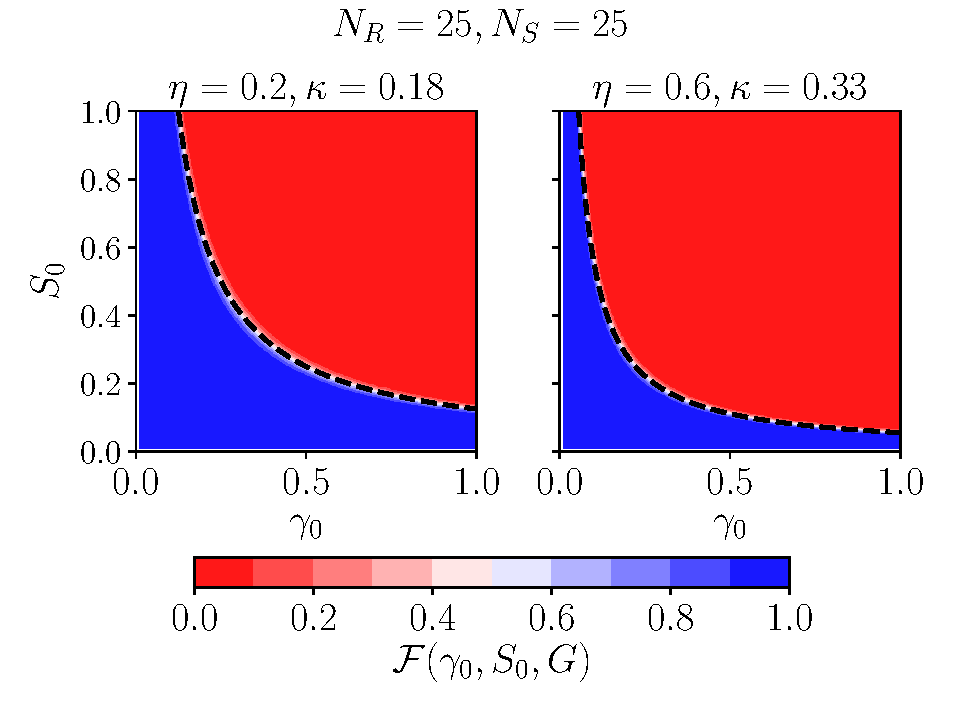
\includegraphics[width=0.7\linewidth]{typical_feasibility_volume}
\caption{Plot of the feasibility region in the absence of syntrophy. The color curve indicates the feasibility function $\mathcal{F}\left((\gamma_0, S_0, \alpha_0=0), G, 0\right)$ for $G_1$, which has a connectance $\kappa_{G}=0.18$ and ecological overlap $\eta_{G}=0.2$ (left) and $G_2$ with $\kappa_G=0.28$ and $\eta_G=0.4$(right). We observe a steep descent which marks a very clear transition from a totally feasible regime to a totally unfeasible regime, which allows us to precisely get the boundary of $\mathcal{F}^{G, 0}_1$. The dashed lines indicate the theoretical predictions.}
\label{fig: typical feasibility region}
\end{figure}
\begin{figure}[h!]
	\captionsetup[subfigure]{captionskip = -165pt, margin = 45pt}
\subfloat[\label{fig: deviation away from theory feasibility fixed nestedness}]{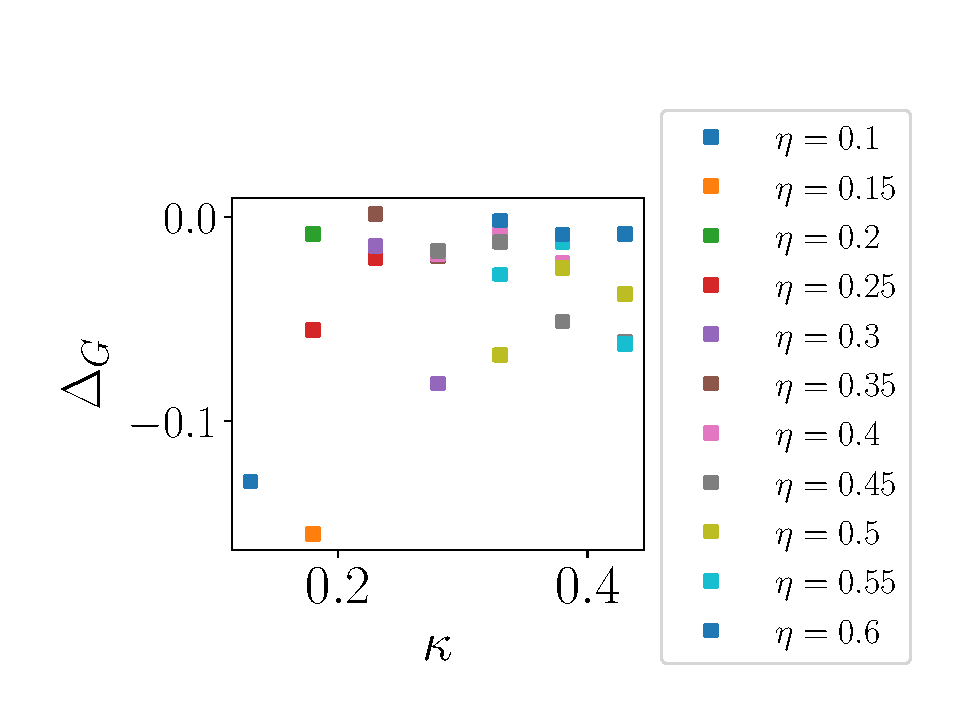
\includegraphics[width=0.49\linewidth]{feasibility_away_from_theory_fixed_nestedness}}
\captionsetup[subfigure]{captionskip = -175pt, margin = 45pt}
\subfloat[\label{fig: deviation away from theory feasibility fixed connectance}]{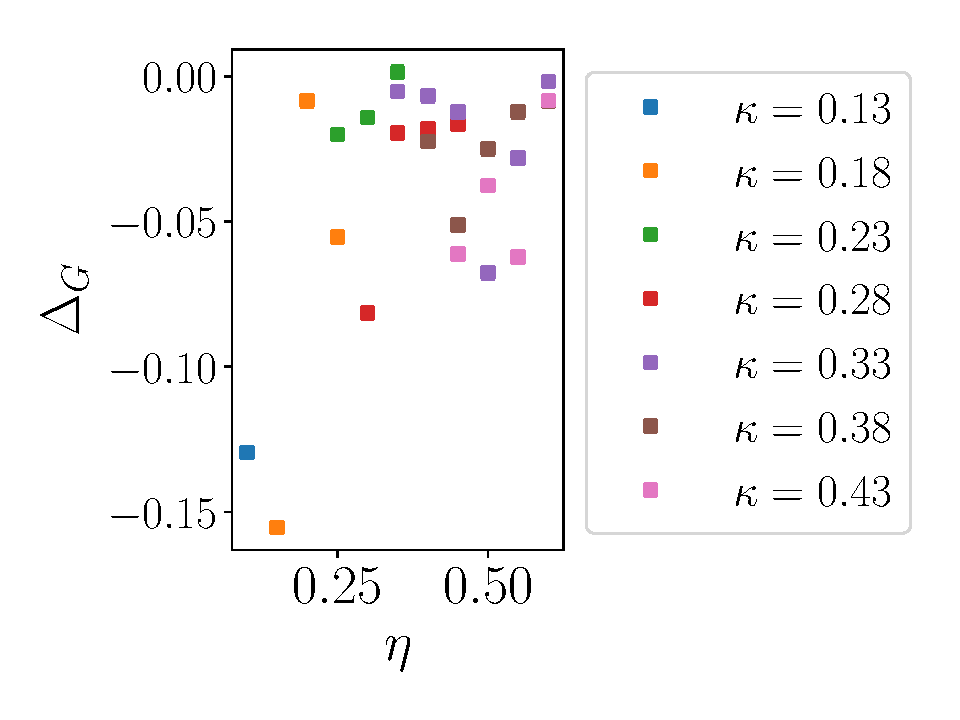
\includegraphics[width=0.49\linewidth]{feasibility_away_from_theory_fixed_connectance}}
\caption{Relative error in the determination of the boundary of $\mathcal{F}^{G,0}_1$ (a) varying connectance at fixed ecological overlap and (b) varying ecological overlap at fixed connectance. The theoretical prediction tends to overestimate the measured value. The larger the ecological overlap or connectance, the better the estimate.}\label{fig: deviation away from theory feasibility}
\end{figure}
\begin{figure}[h!]
\centering
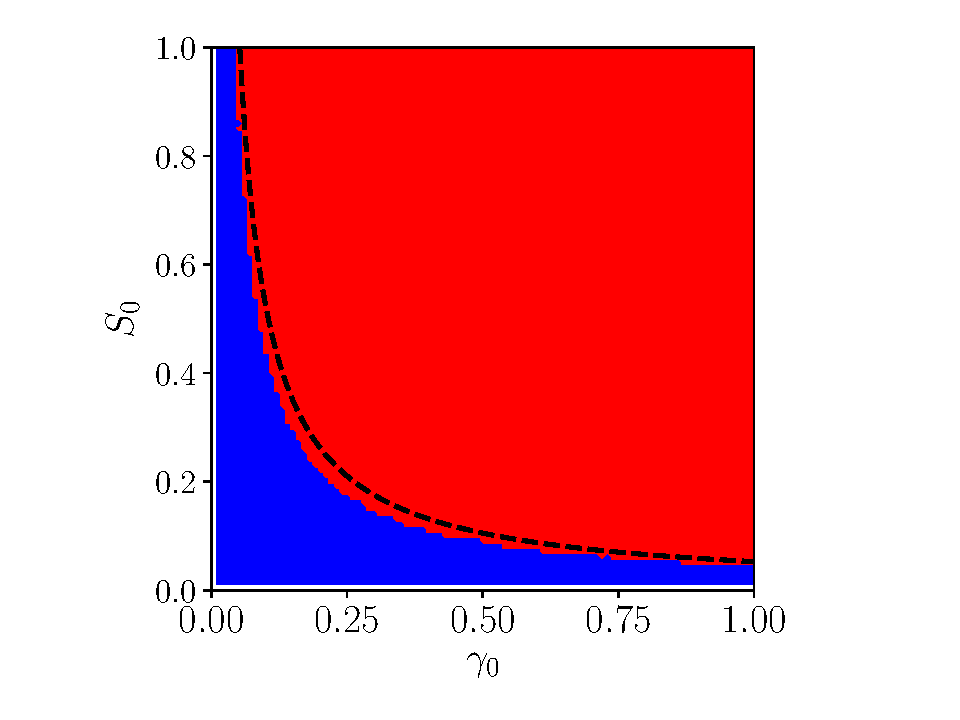
\includegraphics[width=0.6\linewidth]{common_feasibility_volume_no_syntrophy}
\caption{Plot of the common feasibility region. The blue area indicates the common feasibility volume, computed numerically, while the dashed line shows the analytical prediction. Although the match is not as good as before, the relative error is only of the order of $20 \%$. The red part is the area where not all matrices are fully feasible.}
\label{fig: common feasible volume no syntrophy}
\end{figure}
\begin{figure}
\captionsetup[subfigure]{captionskip = -195pt, margin=65pt}
\hspace{-0.2\linewidth}
\subfloat[\label{fig: feasibility results feasibility region eta 0.6 kappa 0.3 NR=25}]{\includegraphics[width=1.4\linewidth]{{feasibility_region_wt_wc_NR25_NS25_Nest0.6_Conn0.3168}.pdf}}

\vspace{-60pt}
\hspace{-0.2\linewidth}
\subfloat[]{\includegraphics[width=1.4\linewidth]{{feasibility_region_wt_wc_NR25_NS25_Nest0.35_Conn0.2208}.pdf}}

\vspace{-60pt}
\hspace{-0.2\linewidth}
\subfloat[]{\includegraphics[width=1.4\linewidth]{{feasibility_region_wt_NR25_NS25_Nest0.15_Conn0.1808}.pdf}}

\caption{Fully feasible region in the $(\gamma_0,S_0) \in [0,1] \times [0,1]$ unit square as a function of syntrophy for different consumption matrices $G$: (a)
$\eta_G=0.6$, $\kappa_G=0.32$, (b) $\eta_G=0.35$, $\kappa_G=0.22$ and (c) $\eta_G=0.15$, $\kappa_G=0.18$.
The white zone corresponds to points that are never fully feasible. The colour of a given point tells until which syntrophy that point is fully feasible, \eg
a light blue point is fully feasible for $0 \leq \alpha_0 \leq \num{9.1e-3}$. The size of the feasibility regions depend heavily on the topology of the matrix, which makes the problem far from trivial.}\label{fig: feasibility results fully feasible volume different consumption matrices}
\end{figure}
\begin{figure}
\centering
\includegraphics[width=0.6\linewidth]{{size_feasibility_region_NR25_NS25_Nest0.25_Conn0.2336}.pdf}
\caption{Decay of the volume of the fully feasible region $\mathcal{F}^{G,A}_1(\alpha_0)$ for a matrix consumption $G$ with ecological overlap $\eta_G=0.25$ and connectance $\kappa_G=0.23$ on a logarithmic scale. The solid lines represent the exponential fit explained in the main text. The four different colors represent the four different structures considered for the syntrophy matrix. The decay of $\text{Vol}(\mathcal{F}^{G,A}_1(\alpha_0))$ seems well approximated by an exponential decay. A random syntrophy matrix (RS scenario) allows for a larger feasibility volume.}
\label{fig: feasibility results typical shrinkage of feasible volume}
\end{figure}
\begin{figure}
\captionsetup[subfigure]{captionskip=-190pt, margin=44pt}
\hspace{-0.05\linewidth}
\subfloat[]{\includegraphics[width=0.55\linewidth]{{feasibility_NR25_NS25_feasibility_decay_rate_fixed_nestedness_fully_connected}.pdf}}
\subfloat[]{\includegraphics[width=0.55\linewidth]{{feasibility_NR25_NS25_feasibility_decay_rate_fixed_connectance_fully_connected}.pdf}}
\caption{Feasibility decay rate $d_F(G,A)$ for $A$ fully connected and $(G,A)\in S_{25}$. (a) $d_F$ as a function of the connectance of $G$ for different fixed ecological overlaps and (b) $d_F$ as a function of the ecological overlap $\eta_G$ for fixed different connectances. A strong trend may be seen: at fixed ecological overlap, $d_F$ decreases with connectance and at fixed connectance it increases with ecological overlap. Since a small $d_F$ allows to sustain a larger syntrophy, microbial communities where syntrophic interactions play a large role will tend to have a high connectance of the consumption matrix and a low ecological overlap.}\label{fig: feasibility results decay rate FC case}
\end{figure}
\begin{figure}
\captionsetup[subfigure]{captionskip=-180pt, margin=44pt}

\vspace{-30pt}
\hspace{-0.03\linewidth}
\subfloat[]{\includegraphics[width=0.53\linewidth]{{feasibility_NR25_NS25_feasibility_decay_rate_dev_away_from_FC_fixed_nestedness_no_release_when_eat}.pdf}}
\subfloat[]{\includegraphics[width=0.53\linewidth]{{feasibility_NR25_NS25_feasibility_decay_rate_dev_away_from_FC_fixed_connectance_no_release_when_eat}.pdf}}

\vspace{-12pt}
\hspace{-0.03\linewidth}
\subfloat[]{\includegraphics[width=0.53\linewidth]{{feasibility_NR25_NS25_feasibility_decay_rate_dev_away_from_FC_fixed_nestedness_optimal_matrix}.pdf}}
\subfloat[]{\includegraphics[width=0.53\linewidth]{{feasibility_NR25_NS25_feasibility_decay_rate_dev_away_from_FC_fixed_connectance_optimal_matrix}.pdf}}

\vspace{-12pt}
\hspace{-0.03\linewidth}
\subfloat[]{\includegraphics[width=0.53\linewidth]{{feasibility_NR25_NS25_feasibility_decay_rate_dev_away_from_FC_fixed_nestedness_random_structure}.pdf}}
\subfloat[]{\includegraphics[width=0.53\linewidth]{{feasibility_NR25_NS25_feasibility_decay_rate_dev_away_from_FC_fixed_connectance_random_structure}.pdf}}
\vspace{-6pt}
\caption{Relative difference of the feasibility decay rate for the considered $A$ scenario compared to the FC null case (Fig.\ref{fig: feasibility results decay rate FC case}) for $N_R=25$ and $N_S=25$. Plots on the first column (a)-(c)-(e) show how that quantity changes with connectance for a given ecological overlap, while plot on the second column (b)-(d)-(f) show how it evolves when ecological overlap is changed and connectance is kept fixed. Different structures of the $A$ matrix are considered: (a)-(b) NIS, (c)-(d) LRI (e)-(f) RS. A positive $y$-coordinate means that for the feasibility decay rate of the current syntrophy scenario is smaller than for the FC case, \ie the system sustains syntrophy better with the considered $A$-structure compared to fully connected. Apart from a few marginal exceptions, the FC scenario is always outperformed by the other scenarios, especially the random structure (RS) case.}\label{fig: feasibility results feasibility decay rate vs matrix structure}
\end{figure}
\begin{figure}[h!]
% \captionsetup[subfigure]{captionskip = -185pt, margin = 195pt}
%
% \hspace{-0.1\linewidth}
% \subfloat[]{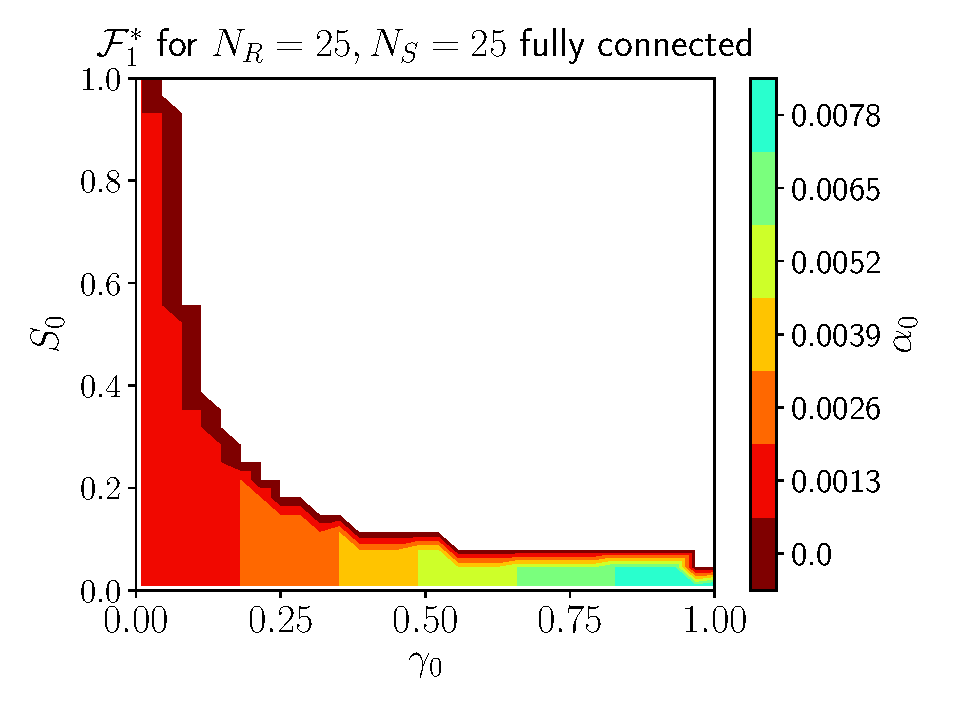
\includegraphics[width=0.6\linewidth]{common_feasibility_volume_NR25_NS25_varying_syntrophy_random_structure}}
% \subfloat[]{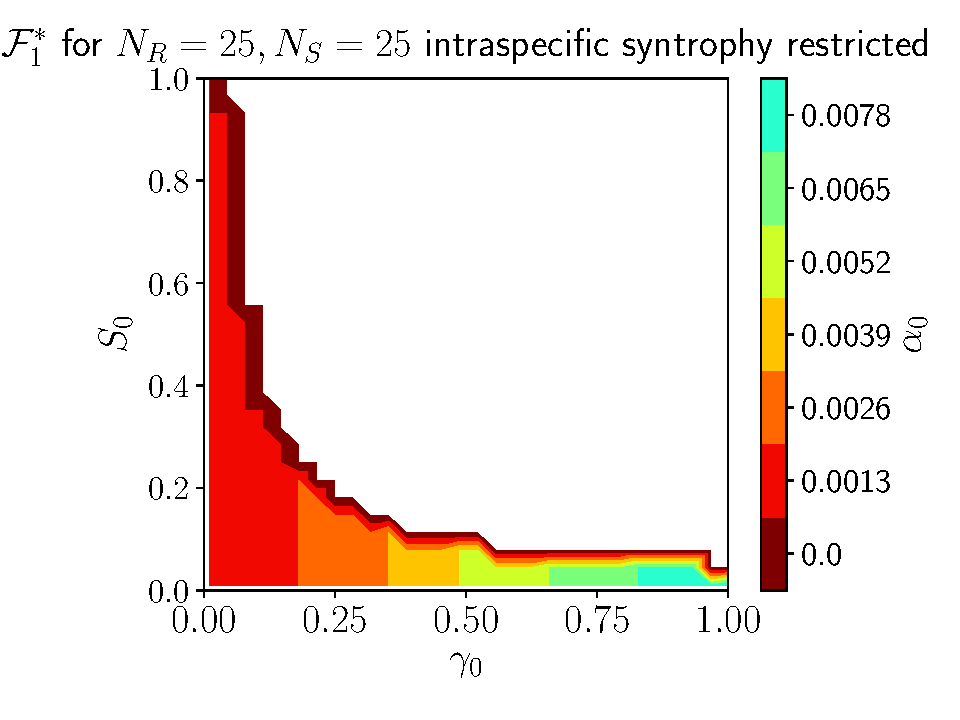
\includegraphics[width=0.6\linewidth]{common_feasibility_volume_NR25_NS25_varying_syntrophy_no_release_when_eat}}
%
% \centering
% \subfloat[]{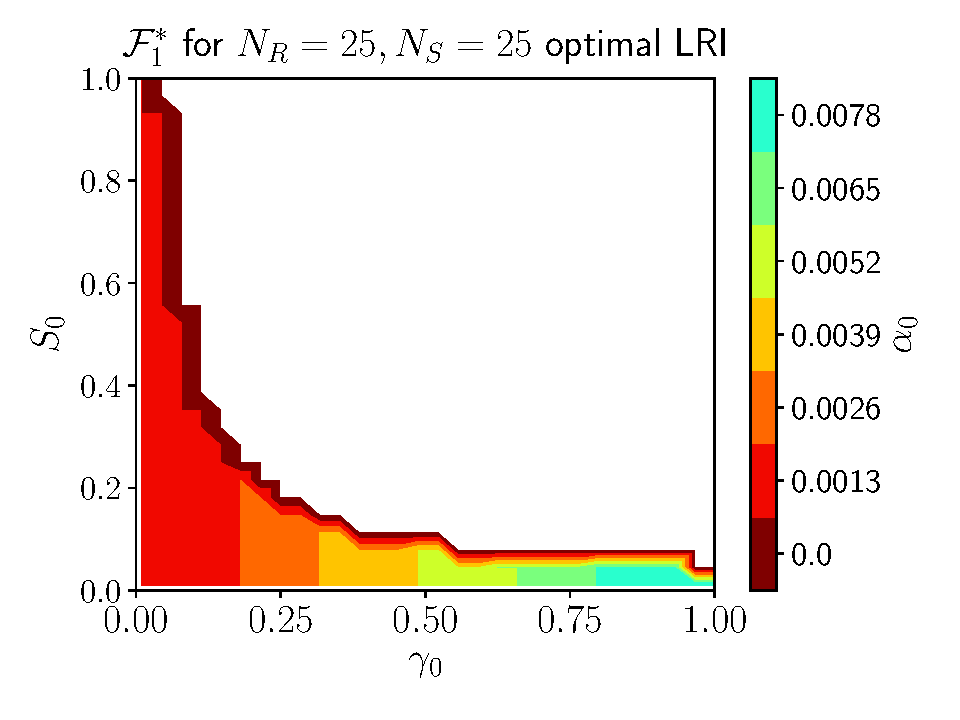
\includegraphics[width=0.6\linewidth]{common_feasibility_volume_NR25_NS25_varying_syntrophy_optimal_matrix}}
\hspace{-0.2\linewidth}
\includegraphics[width=1.4\linewidth]{{common_feasibility_region_NR25_NS25}.pdf}

\caption[caption for LOF]{Surface plot of the fully feasible volume $\mathcal{F}^{S_{25}}_1(\alpha_0)$. The color bar on the side indicates the value of $\alpha_0$ to which the surface corresponds. The white part of the plot corresponds to points that \important{never} are fully feasible. Note that even though it is not very clear on the figure $\mathcal{F}_1^{S_{25}}(\alpha_0^+) \subset \mathcal{F}_1^{S_{25}}(\alpha_0^-) \ \forall \alpha_0^+ > \alpha_0^-$, \ie the common fully feasible region of higher syntrophy is included in the one of lower syntrophy. The different subplots correspond to the different structures of the syntrophy matrix.} \label{fig: results feasibility cfv variation with syntrophy}
\end{figure}
\begin{figure}
\centering
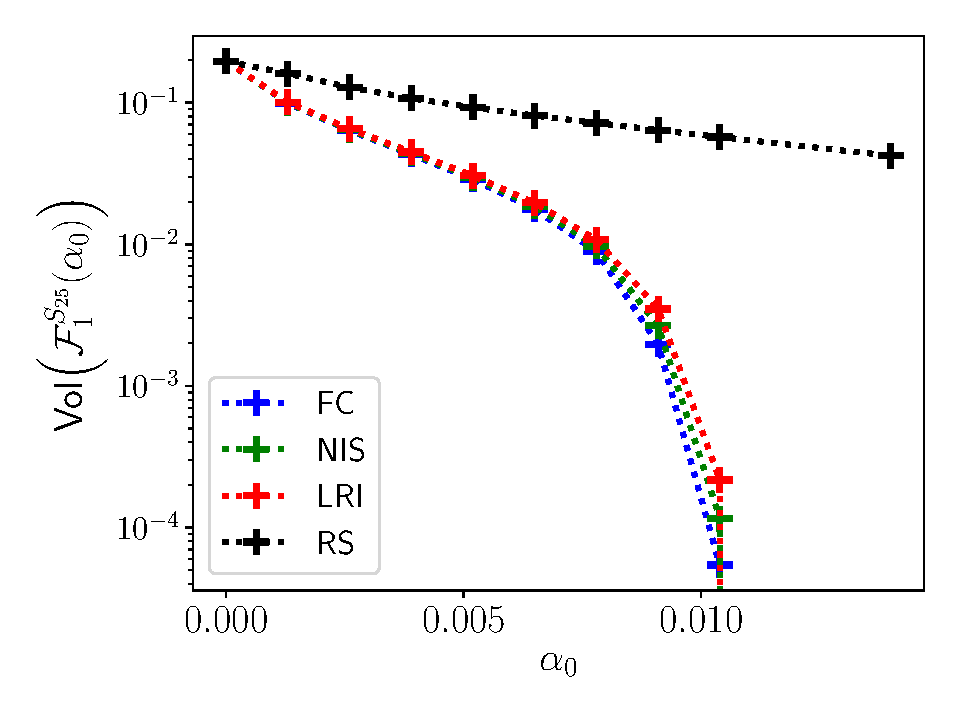
\includegraphics[width=0.65\linewidth]{common_feasibility_volume_NR25_NS25}
\caption{Volume of the common feasibility region $\mathcal{F}^{S_{25}}_1(\alpha_0)$ as a function of syntrophic interaction strength $\alpha_0$ (plotted on logarithmic scale). While the FC, NIS and LRI cases offer similar results, the RS scenario outperforms all of them. An exponential fit (Eq.\ref{eq: feasibility results fit feasible volume}) allows to measure a global $d_F$ for each of the four scenarios. The global decay feasibility rate of the RS scenario is 2.5 times smaller than the others.}\label{fig: feasibility results volume of cfr depending on syntrophy}
\end{figure}

\begin{figure}
\vspace{-120pt}
\hspace{-0.05\linewidth}
\subfloat[\label{fig: feasibility results feasibility region eta 0.6 kappa 0.3}]{\includegraphics[width=1.1\linewidth]{{feasibility_region_wt_NR50_NS25_Nest0.6_Conn0.3344}.pdf}}

\vspace{-28pt}
\hspace{-0.05\linewidth}
\subfloat[]{\includegraphics[width=1.1\linewidth]{{feasibility_region_wt_NR50_NS25_Nest0.35_Conn0.2296}.pdf}}

\vspace{-28pt}
\hspace{-0.05\linewidth}
\subfloat[\label{fig: feasibility results feasibility region eta 0.15 kappa 0.12}]{\includegraphics[width=1.1\linewidth]{{feasibility_region_wt_NR50_NS25_Nest0.15_Conn0.12}.pdf}}
\vspace{-12pt}
\caption{Surface colour plot of the fully feasible region $\mathcal{F}_1^{G,A}\left(\alpha_0\right)$ as a function of the syntrophy $\alpha_0$ for the case $N_R=50$, with different structures of $A$: fully connected (left column), no intraspecific syntrophy (middle) and LRI matrix (right). The rows correspond to different choices of the consumption matrix $G$: (a) $\eta_G=0.6$ and $\kappa_G=0.33$, (b) $\eta_G=0.35$ and $\kappa_G=0.23$, (c) $\eta_G=0.15$ and $\kappa_G=0.12$. These are matrices with similar properties than  Fig.\ref{fig: feasibility results fully feasible volume different consumption matrices}, except that the number of resources is here doubled. This affects $\mathcal{F}_1^{G,A}\left(\alpha_0\right)$ quite drastically.}\label{fig: feasibility results typical feasible volumes NR=50 NS=25}
\vspace{-60pt}
\end{figure}
\begin{figure}[h!]
\captionsetup[subfigure]{captionskip = -185pt, margin = 195pt}

\hspace{-0.1\linewidth}
\subfloat[]{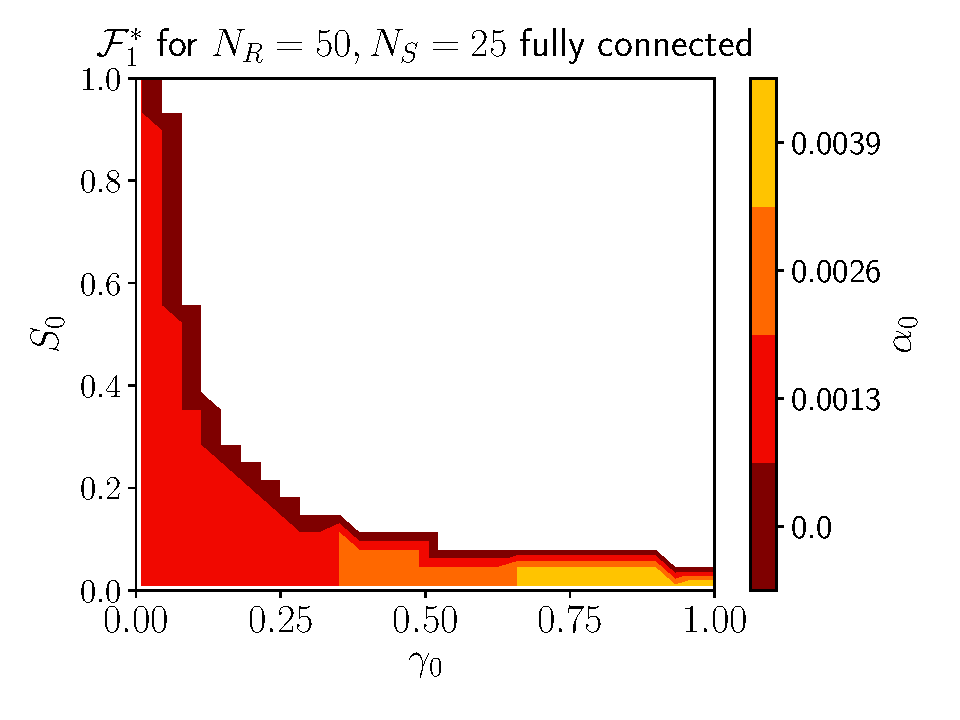
\includegraphics[width=0.6\linewidth]{common_feasibility_volume_NR50_NS25_varying_syntrophy_random_structure}}
\subfloat[]{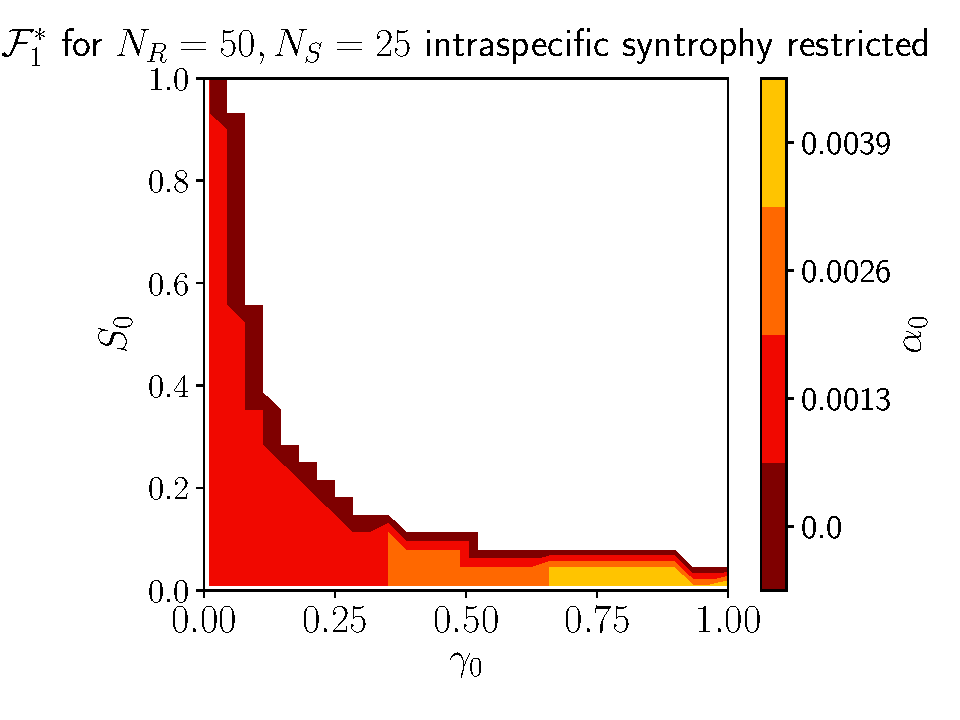
\includegraphics[width=0.6\linewidth]{common_feasibility_volume_NR50_NS25_varying_syntrophy_no_release_when_eat}}

\centering
\subfloat[]{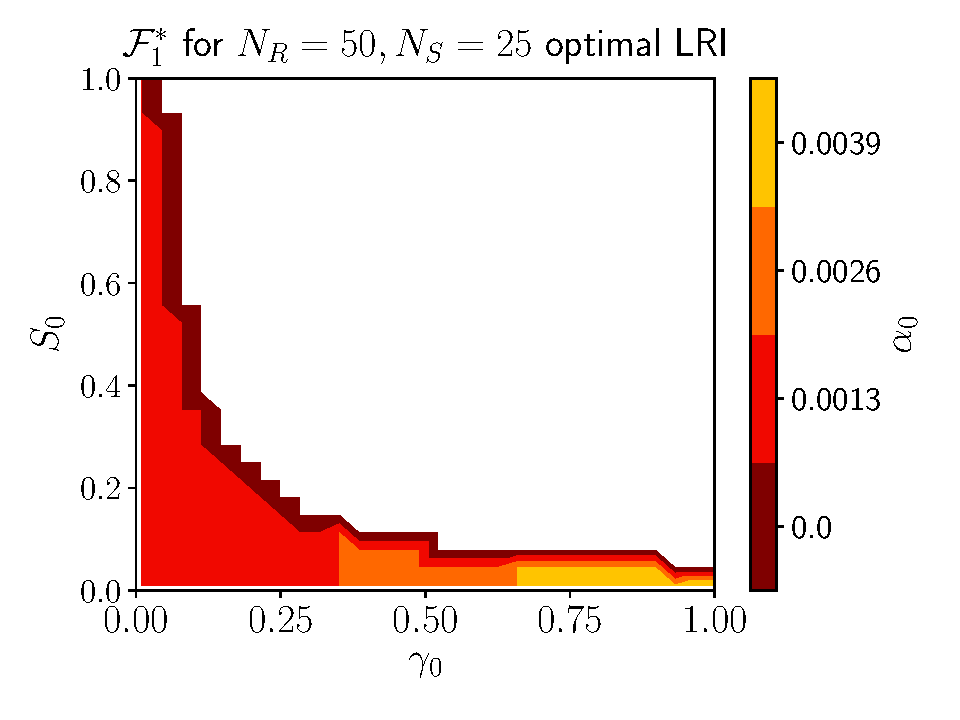
\includegraphics[width=0.6\linewidth]{common_feasibility_volume_NR50_NS25_varying_syntrophy_optimal_matrix}}
\caption{Common feasibility region $\mathcal{F}_1^{S_M}\left(\alpha_0\right)$ for $N_R=50$ and $N_S=25$, to compare with \ref{fig: results feasibility cfv variation with syntrophy}. We considered different structures of the syntrophy matrix: (a) fully connected, (b) intraspecific syntrophy restricted and (c) LRI matrix. As the number of resources increases, the feasibility volume for a given $\alpha_0$ decreases.}\label{fig: feasibility results common feasibility region NR=50 NS=25}
\end{figure}

\begin{figure}
\vspace{-84pt}
\captionsetup[subfigure]{captionskip=-202pt, margin=45pt}
\hspace{-0.1\linewidth}
\subfloat[]{\includegraphics[width=0.6\linewidth]{{feasibility_decay_rate_50_vs_25_fixed_connectance_fully_connected}.pdf}}
\subfloat[]{\includegraphics[width=0.6\linewidth]{{feasibility_decay_rate_50_vs_25_fixed_nestedness_fully_connected}.pdf}}

\hspace{-0.1\linewidth}
\subfloat[]{\includegraphics[width=0.6\linewidth]{{feasibility_decay_rate_50_vs_25_fixed_connectance_no_release_when_eat}.pdf}}
\subfloat[]{\includegraphics[width=0.6\linewidth]{{feasibility_decay_rate_50_vs_25_fixed_nestedness_no_release_when_eat}.pdf}}

\hspace{-0.1\linewidth}
\subfloat[]{\includegraphics[width=0.6\linewidth]{{feasibility_decay_rate_50_vs_25_fixed_connectance_optimal_matrix}.pdf}}
\subfloat[]{\includegraphics[width=0.6\linewidth]{{feasibility_decay_rate_50_vs_25_fixed_nestedness_optimal_matrix}.pdf}}

\vspace{-12pt}
\hspace{-0.1\linewidth}
% \subfloat[]{\includegraphics[width=0.6\linewidth]{{feasibility_decay_rate_50_vs_25_fixed_connectancerandom_structure}.pdf}}
% \subfloat[]{\includegraphics[width=0.6\linewidth]{{feasibility_decay_rate_50_vs_25_fixed_nestednessrandom_structure}.pdf}}

\caption{Ratio of the feasibility decay rates at $N_R=25$ and at $N_R=50$ as a function of the consumption matrix properties. A $y$-axis larger than $1$ means $d_F(N_R=25)$ is larger than $d_F(N_R=50)$, which means the system endures the addition of syntrophic interaction better at $N_R=50$. We considered the four usual $A$ scenarios (a)-(b) FC, (c)-(d) NIS, (e)-(f) LRI and (g)-(h) RS. Increasing the number of resources in the system does not allow microbial communities to be ``more feasible'' as syntrophy increases: on average $d_F$ is unchanged by doubling the number of resources. A detailed on how the consumption matrix properties, at least connectance and ecological overlap, or the $A$-scenario precisely modify the improvement is difficult to draw from this data.\textbf{TO DO: put also the one for random structure}}
\label{fig: feasibility results feasibility decay rate NR=50 NS=25}
\end{figure}
\end{document}





\end{document}
